\documentclass[11pt,a4paper]{article}

%used packages
\usepackage{graphicx}
\usepackage[dutch]{babel} 
\usepackage{scrextend}
\usepackage{enumitem}
\usepackage{listings}
\usepackage{float}
\usepackage{titlesec}
\usepackage[table,xcdraw]{xcolor}
\usepackage{fancyhdr}
\usepackage{lastpage}
\usepackage{xcolor}
\usepackage{listings}
\usepackage{hyperref}
\usepackage{amsmath}
 

%Document settings
\raggedbottom
\graphicspath{ {images/} }
\setlength{\parindent}{0em}
\setlength{\parskip}{1em}

%Custom commando's
\newcommand\litem[1]{\item{\bfseries#1.\space}}
\newcommand\tabelkleur{\rowcolor[HTML]{FFCC67}}


%Custum Variables
\def\auteureen{Roy Buitenhuis, 0895833}
\def\auteurtwee{Tim van Broekhoven, 0893122}
\def\titel{Verslag TDS01} 
\def\datum{\today}
\def\versie{0.1}
\def\status{concept}
\def\subtitel{Plan van aanpak}
\def\bedrijf{}
\def\tabelkleur{FFCC67}

%Settings for Footer and Header
\pagestyle{fancy}
\fancyhf{}
\rhead{\subtitel}
\lhead{\titel}
\lfoot{\datum}
\rfoot{Pagina \thepage \hspace{1pt} /  \pageref{LastPage}}

%Settings for document spacing
\titlespacing{\section}{0pt}{*0}{*0}
\titlespacing{\subsection}{0pt}{*0}{*0}
\titlespacing{\subsubsection}{0pt}{*0}{*0}

%Settings for code sinppeds
\lstset{basicstyle=\ttfamily,
	showstringspaces=false,
	commentstyle=\color{red},
	keywordstyle=\color{blue},
	columns=fullflexible,
	frame=single,
	breaklines=true,
	postbreak=\mbox{\textcolor{red}{$\hookrightarrow$}\space},
}

\begin{document}
	
	\begin{titlepage}
		
		\centering
		{\huge\bfseries \titel \par}
		
		\vspace{1cm}
		{\Large\itshape \auteureen \par}
		{\Large\itshape \auteurtwee \par}
		\vspace{1cm}
		{\Large\itshape versie \versie\par}
				
		\vfill
		Vak:\par
		TDS01
		
		\vfill
		{\large \datum \par}
	\end{titlepage}

	\section{Samenvatting}

Het vak Training Digitale Signaalbewerking (TDS02) leert de studenten van de minor 'Embedded systems' om de theorie die hoort bij Digitale Signaal Bewerking (DSB) in de praktijk te brengen. Het doel van digitale signaalbewerking is om met de informatie van het ingangssignaal een uitgangssignaal te produceren die bruikbaar is voor een bepaalde toepassing. 

Omdat digitale filters veel gebruikt worden voor toepassingen in DSB, worden de studenten gevraagd om twee verschillende soorten filters te bouwen voor dit vak: Een 'finite impulse response' (FIR) filter en een 'infinite impulse response' (IIR) filter. 

De requirements  voor deze assignments krijgen de studenten van hun docenten. Voor onze FIR assignment moesten we een hoogdoorlaatfilter maken en voor de IIR assignment moesten we een bandstopfilter. 
	
De werkwijze van het uitvoeren van de assignments begint met het maken van de filter in matlab. Vervolgens kunnen de coefficienten door matlab geproduceerd worden die nodig zijn voor de digitale filter. Met die coefficienten kan de code voor de filter worden geschreven in CCS. Die code moet vervolgens op het DSP development-bordje worden geupload. Een pulsgenerator wordt dan aangesloten op het ingangssignaal van dat bordje en de audio-ingang van een computer wordt aangesloten op de het uitgangssignaal van het development-bordje, waardoor op die computer een scoopbeeld gegenereerd kan worden m.b.v. software voor scoopbeelden. 

De grootste uitdaging van deze assignments bleek te zitten in de wiskundige formules die we in de code moesten toepassen. Vooral voor de IIR filter was dit een uitdaging en is er helaas niet volledig voldaan aan de eisen die door de docenten gesteld zijn. 
	
De grootste uitdaging van deze assignments bleek te zitten in de wiskundige formules die we in de code moesten toepassen. Vooral voor de IIR filter was dit een uitdaging en is er helaas niet volledig voldaan aan de eisen die door de docenten gesteld waren. 

Kwa code is een deel van de CXX stof meegenomen. Zo hebben we een struct waar de staat en informatie over de buffers van de filters in wordt opgeslagen. Daar kunnen vervolgens bewerkingen op worden gedaan. Zoal het opslaan van nieuwe samples en het berekenen van een outputsample. Dit maakte de code beter leesbaar en herbruikbaar.
	 
		
	
	\clearpage
	
	\tableofcontents
	
	\clearpage
	
	\listoffigures
	
	\clearpage
	\listoftables
	
	\clearpage
	
	\section{Versiehistorie}
	\begin{table}[H]
		\centering
		\label{Versiehistorie}
		\begin{tabular}{|p{1cm}|p{2cm}|p{6cm}|p{2cm}|}
			\hline
			\rowcolor[HTML]{FFCC67}
			\textbf{Versie} & \textbf{Datum} & \textbf{Wijzigingen} & \textbf{Auteur} \\ \hline
			0.1    & 25-10-2017 & Template    & Tim \\ \hline
			0.2	   & 31-10-2017 & Oplevering eerste versie  & Groep \\ \hline
			&       &             &        \\ \hline
		\end{tabular}
		\caption {Versiehistorie} \label{tab:title} 
	\end{table}	


	\section{Introductie}
		\subsection{Het vak}
		TDS02 is een van de vakken die tijdens de minor 'Embedded Systems' wordt gegeven. Het vak bestaat voornamelijk uit practicum assignments die de studenten in groepjes van twee dienen te voltooien. In de eerste weken begint de les met een uitleg van de docent over de theorie achter deze assignments, die het doel hebben om de studenten te trainen in digitale signaalbewerking. Om de assignments te voltooien dienen de studenten gebruik te maken van de 'C5505 eZdsp Development Tool' van Texas Instruments.
		
		\subsection{Introductie DSP}
		Volgens Analog Devices \cite{analog} is een DSP een processor die een gedigitaliseerd signaal als geluid, video, temperatuur of positie op wiskundige wijze manipuleerd. Analog Devices ligt toe dat een DSP wordt ontworpen om berekeningen als "optellen", "aftrekken", "vermenigvuldigen" en "delen" in korte tijd te kunnen voltooien. Het doel van deze berekeningen is om met de informatie van het ingangssignaal een uitgangssignaal te produceren die bruikbaar is voor een bepaalde toepassing. 
		
		\subsection{Digitale filter}
		Volgens Steven W. Smith \cite{DSPguide} bewerkt een digitale filter een digitaal en tijd-discreet signaal om bepaalde frequenties uit dat signaal te verzwakken. In de telecomunicatie wordt bijvoorbeeld het signaal van het bericht gemengd met de draaggolf van het bericht. Om dit bericht vervolgens uit te kunnen lezen moet er een filter gebruikt worden om de frequenties van het draaggolfsignaal eruit te filteren. Dit kan gedaan worden m.b.v. een analoge of digitale filter. Analoge filters hebben een groot bereik met zowel amplitude als frequentie. Ook kunnen analoge filters heel precies worden ingesteld. Digitale filters hebben echter meer voordelen dan analoge filters. Digitale filters zijn flexibel, betrouwbaar, makkelijk in schaal te vergroten en om de complexiteit van een filter te verhogen moet de software worden aangepast i.p.v. de hardware. 
		
Om analoge signalen digitaal te kunnen filteren moeten de signalen worden gesampled en gekwantificeerd worden. Hierdoor ontstaat een digitaal en tijd-discreet signaal. 

Filters kunnen gezien worden als een overdrachtsfunctie:
 
\[
    H(s) = \frac{Y(s)}{X(s)}
\]	

Waarbij X(s) de input is van de filter en Y(s) de uitgang van de filter. 

De overdrachtsfunctie kan gespecificeerd worden in het frequentiedomein en is een wiskundige formule die het gedrag van de filter omschrijft.  

		
	\subsection{De opdracht}		
		
	\section{Ontwerp en realisatie FIR filter}

\subsection{What where the requirements for this filter?}
Het filter dat moest worden gerealiseerd is een hoogdoorlaatfilter met een cut-off frequentie van 1500 Hertz. 
Het filter moest een minimale orde van 20 hebben. Er moest gebruik worden gemaakt van het blackmann window.

\subsection{How are the coefficients determined?}
Als samplerate is gekozen voor 8000 hertz. Dit is genoeg om de werking van het filter te kunnen aantonen, maar maakt het filter ongeschikt voor toepassingen in geluid. 
Kwa orde is gekozen voor een 100'ste orde filter. Dit hebben we gedaan om de lijn van het filter stijler te maken.
Het filter is gequantificeerd voor fixed-point getallen. Dit omdat de EzDSP beter presteerd met fixed-point getallen.


    \begin{enumerate}[label=\emph{\alph*)}]
        \litem{orde} 100'ste
        \litem{type} FIR: window
        \litem{window} Blackmann
        \litem{Fsample} 8kHz
        \litem{Fcutoff} 1500Hertz
    \end{enumerate}

    \subsection{Matlab}
    
    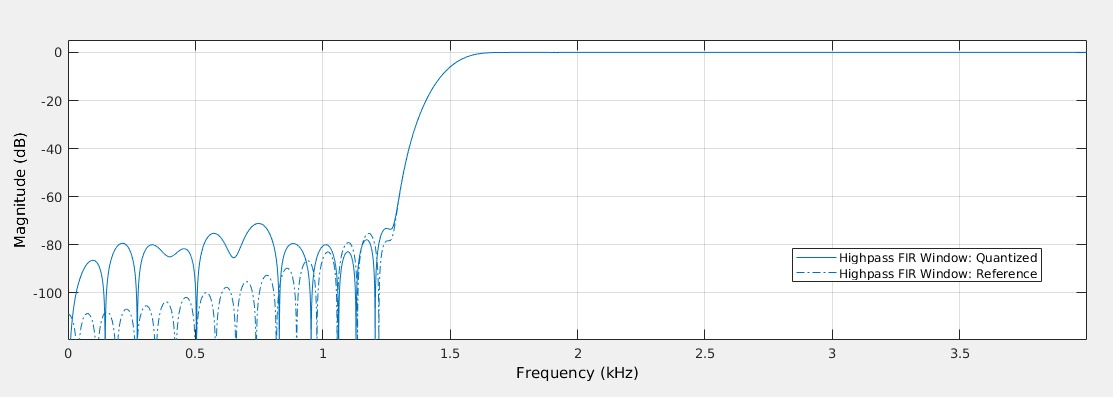
\includegraphics[width=0.80\textwidth]{firMatlab}\par\vspace{1cm}
    \clearpage
    \subsection{Code}

    \subsubsection{de main code.}
        
        \begin{lstlisting}[language=c]
#include <stdio.h>
#include <usbstk5505.h>
#include <usbstk5505_led.h>
#include <csl_intc.h>

#include "aic3204.h"
#include "fdacoefs.h"
#include "fir_buffer.h"

#define SAMPLES_PER_SECOND 8000 // possible values: 48000, 24000, 16000, 12000, 9600, and 8000
#define ADC_GAIN  0// range: 0dB to 48 dB
#define DAC_GAIN 0// range: -6dB to 29dB


extern void VECSTART(void);

FIRBuffer *buffer;
interrupt void I2S0receive() {

    fir_buffer_store_sample(buffer, AIC3204_readLeft());
    AIC3204_writeLeft(fir_buffer_output_sample(buffer, COEFFICIENTS));

}

int main(void) {
    buffer = fir_buffer_new(COEFFICIENTS_LENGTH);

    USBSTK5505_init();
    AIC3204_init(SAMPLES_PER_SECOND, ADC_GAIN, DAC_GAIN);
    IRQ_setVecs((Uint32)(&VECSTART));
    IRQ_plug(PROG1_EVENT,&I2S0receive);
    IRQ_enable(PROG1_EVENT);
    IRQ_globalEnable();

    while(1);
}
            \end{lstlisting}
            \clearpage	
        
            \subsubsection{De header van de fir buffer}
            \begin{lstlisting}[language=c]
#ifndef __FIR_BUFFER__
#define __FIR_BUFFER__

#include <csl_intc.h>

typedef struct {
    int size;
    Int16 *buffer;
    int currentBufferIndex;
} FIRBuffer;

FIRBuffer * fir_buffer_new(int size);
void fir_buffer_store_sample(FIRBuffer *buffer, Int16 sample);
Int16 fir_buffer_output_sample(FIRBuffer *buffer, const Int16 *coefficients);

#endif//__FIR_BUFFER__
        
            \end{lstlisting}
            \clearpage
        
            \subsubsection{Code van de fir buffer}
            \begin{lstlisting}[language=c]
#include <stdlib.h>
#include "fir_buffer.h";

FIRBuffer * fir_buffer_new(int size) {
    FIRBuffer *firBuffer = (FIRBuffer *)malloc(sizeof(FIRBuffer));
    //TODO: Still have to solve potential nullpointer issues.

    firBuffer->size = size;
    firBuffer->buffer = malloc(sizeof(Int16) * size);
    firBuffer->currentBufferIndex = 0;

    return firBuffer;
}

void fir_buffer_store_sample(FIRBuffer *buffer, Int16 sample) {
    buffer->currentBufferIndex += 1;

    if(buffer->currentBufferIndex == buffer->size) {
            buffer->currentBufferIndex = 0;
    }

    buffer->buffer[buffer->currentBufferIndex] = sample;
}

Int16 fir_buffer_output_sample(FIRBuffer *buffer, const Int16 *coefficients) {
    Int32 output = 0;
    int k;
    for(k = 0; k < buffer->size; k++){
        int bufferIndex = buffer->currentBufferIndex - k;
        if(bufferIndex < 0){
            bufferIndex += buffer->size;
        }
        output += (Int32)coefficients[k] * (Int32)buffer->buffer[bufferIndex];
    }

    return((Int16)(output >> 15));
}
            \end{lstlisting}
            \clearpage	
        
            \begin{lstlisting}[language=c]
/*
* Filter Coefficients (C Source) generated by the Filter Design and Analysis Tool
* Generated by MATLAB(R) 9.2 and the DSP System Toolbox 9.4.
* Generated on: 09-Oct-2017 11:48:44
*/

/*
* Discrete-Time FIR Filter (real)
* -------------------------------
* Filter Structure  : Direct-Form FIR
* Filter Length     : 101
* Stable            : Yes
* Linear Phase      : Yes (Type 1)
* Arithmetic        : single
*/
/*
* Warning - Filter coefficients were truncated to fit specified data type.  
*   The resulting response may not match generated theoretical response.
*   Use the Filter Design & Analysis Tool to design accurate
*   int16 filter coefficients.
*/
#include <csl_intc.h>
#define COEFFICIENTS_LENGTH 101

const Int16 COEFFICIENTS[COEFFICIENTS_LENGTH] = {
0,      0,      0,      1,      1,     -1,     -3,     -2,      4,
7,      0,    -12,    -12,      8,     25,     12,    -26,    -40,
0,     55,     49,    -31,    -94,    -41,     88,    131,      0,
-170,   -147,     90,    266,    115,   -238,   -350,      0,    443,
381,   -233,   -686,   -298,    626,    938,      0,  -1271,  -1159,
767,   2541,   1311,  -3664,  -9621,  20480,  -9621,  -3664,   1311,
2541,    767,  -1159,  -1271,      0,    938,    626,   -298,   -686,
-233,    381,    443,      0,   -350,   -238,    115,    266,     90,
-147,   -170,      0,    131,     88,    -41,    -94,    -31,     49,
55,      0,    -40,    -26,     12,     25,      8,    -12,    -12,
0,      7,      4,     -2,     -3,     -1,      1,      1,      0,
0,      0
};	
            \end{lstlisting}
            \clearpage
        
        
            \subsection{Het resultaat}
            
    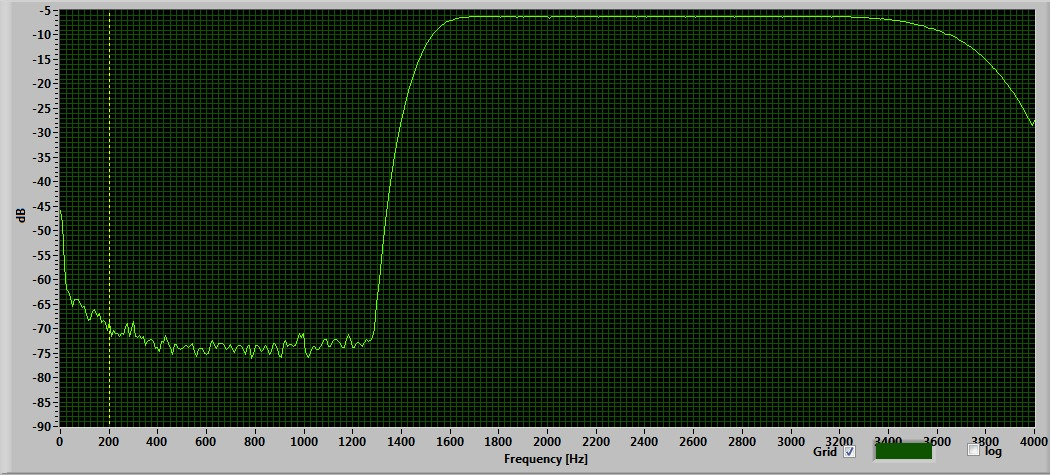
\includegraphics[width=0.80\textwidth]{FIRrealisatie}\par\vspace{1cm}            
            
            \clearpage
            
	\section{Ontwerp en realisatie IIR filter}

\subsection{Requirements IIR filter}
Het IIR filter moet een Band-Stop filter worden. De minimale orde die verwacht wordt is er een van 20. Het filter moet alle frequenties tussen 800 en 1000 hertz dempen. Het type Chebyshev I zal worden toegepast.
\subsection{Coefficienten bepalen}

\begin{enumerate}[label=\emph{\alph*)}]
    \litem{Orde} teruggeschroeft naar 4 om het filter met een elkele sectie stabiel te krijgen.
    \litem{Fsample} teruggeschroeft om het filter stabiel te krijgen.
    \litem{Fixed-point} getallen gebruikt omdat deze geschikt zijn voor de EzDSP. Deze bevat voor Floating-point getallen namelijk geen hardware ondersteuning.
\end{enumerate}

Er drijgde een gebrek aan tijd tijdens het uitvoeren van de laatste opdracht, hierdoor was het niet meer mogelijk om ondersteuning te maken voor een filter dat bestaat uit meerdere secties. 
Daarop is in oveleg met Dhr. Broeders besloten om een filter te maken dat uit een enkele sectie bestaat. Hiervoor hebben we de orde echter moeten terugschroeven, maar dit was dit geval geen probleem mits dit in het verslag werd beschreven. 

\subsection{Matlab}

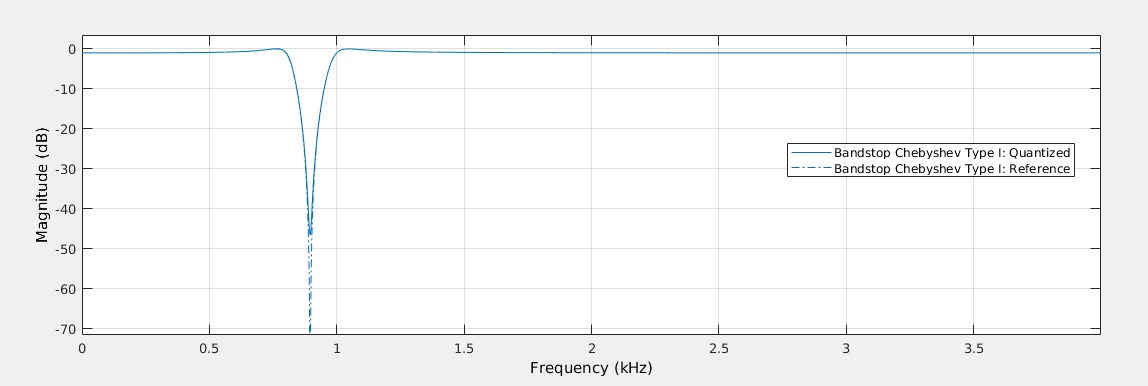
\includegraphics[width=0.80\textwidth]{iirMatlab}\par\vspace{1cm}		
\clearpage
\subsection{Code}

\subsubsection{de main code.}
\begin{lstlisting}[language=c]
#include <stdio.h>
#include <usbstk5505.h>
#include <usbstk5505_led.h>
#include <csl_intc.h>
#include <iir_buffer.h>
#include "aic3204.h"
#include "iir_fdacoefs3.h"

#define SAMPLES_PER_SECOND 8000 // possible values: 48000, 24000, 16000, 12000, 9600, and 8000
#define ADC_GAIN  0// range: 0dB to 48 dB
#define DAC_GAIN 0// range: -6dB to 29dB


extern void VECSTART(void);

 
IIRBuffer *buffer;
interrupt void I2S0receive() {
iir_buffer_store_sample(buffer, AIC3204_readLeft());
AIC3204_writeLeft(iir_buffer_output_sample(buffer, DEN, NUM));

}

int main(void) {
buffer = iir_buffer_new(COEFFICIENTS_LENGTH, 1);

USBSTK5505_init();
AIC3204_init(SAMPLES_PER_SECOND, ADC_GAIN, DAC_GAIN);
IRQ_setVecs((Uint32)(&VECSTART));
IRQ_plug(PROG1_EVENT,&I2S0receive);
IRQ_enable(PROG1_EVENT);
IRQ_globalEnable();

while(1);
}
\end{lstlisting}
\clearpage

\subsubsection{IIR buffer header}
\begin{lstlisting}[language=c]
#ifndef __IIR_BUFFER__
#define __IIR_BUFFER__

#include <csl_intc.h>

typedef struct {
int size;
int sections;
Int16 *buffer;
Int32 *outputBuffer;
int currentBufferIndex;
} IIRBuffer;

IIRBuffer * iir_buffer_new(int size, int sections);
void iir_buffer_store_sample(IIRBuffer *buffer, Int16 sample);
Int16 iir_buffer_output_sample(IIRBuffer *buffer, const Int16 *denominator, const Int16 *numerator);

#endif//__IIR_BUFFER__
    
\end{lstlisting}
\clearpage

\subsubsection{IIR buffer source}
\begin{lstlisting}[language=c]
#include <iir_buffer.h>
#include <stdlib.h>

Int32 direct_form_1(IIRBuffer *buffer, Int32 input, const Int16 *denominator, const Int16 *numerator) {
Int32 output = input;
int k;
for(k = 0; k < buffer->size; k++){
    int bufferIndex = buffer->currentBufferIndex - k;
    if(bufferIndex < 0){
        bufferIndex += buffer->size;
    }

    output += (Int32)numerator[k] * (Int32)buffer->buffer[bufferIndex];
}

int i;
for(i = 1; i < buffer->size; i++) {
    int bufferIndex = buffer->currentBufferIndex - i;
    if(bufferIndex < 0){
        bufferIndex += buffer->size;
    }

    output -= (Int32)denominator[i] * (Int32)buffer->outputBuffer[bufferIndex];
}
return output;
}

IIRBuffer * iir_buffer_new(int size, int sections) {
IIRBuffer *iirBuffer = (IIRBuffer *)malloc(sizeof(IIRBuffer));
//TODO: Still have to solve potential nullpointer issues.

iirBuffer->size = size;
iirBuffer->sections = sections;
iirBuffer->buffer = malloc(sizeof(Int16) * size);
iirBuffer->outputBuffer = malloc(sizeof(Int32) * size);

int i;
for(i = 0; i < size; i++) {
    iirBuffer->buffer[i] = 0;
    iirBuffer->outputBuffer[i] = 0;
}

iirBuffer->currentBufferIndex = 0;

return iirBuffer;
}

void iir_buffer_store_sample(IIRBuffer *buffer, Int16 sample) {
buffer->currentBufferIndex += 1;

if(buffer->currentBufferIndex == buffer->size) {
        buffer->currentBufferIndex = 0;
}

buffer->buffer[buffer->currentBufferIndex] = sample;
}

Int16 iir_buffer_output_sample(IIRBuffer *buffer, const Int16 *denominator, const Int16 *numerator) {
Int32 output = 0;

output += direct_form_1(buffer, output, denominator, numerator);

buffer->outputBuffer[buffer->currentBufferIndex] = output >> 13;
return((Int16)(output>>13));
}
\end{lstlisting}
\clearpage

\subsubsection{IIR coefficients}
\begin{lstlisting}[language=c]
/*
* Filter Coefficients (C Source) generated by the Filter Design and Analysis Tool
* Generated by MATLAB(R) 9.2 and the DSP System Toolbox 9.4.
* Generated on: 23-Oct-2017 14:07:54
*/

/*
* Discrete-Time IIR Filter (real)
* -------------------------------
* Filter Structure    : Direct-Form I
* Numerator Length    : 5
* Denominator Length  : 5
* Stable              : Yes
* Linear Phase        : No
* Arithmetic          : fixed
* Numerator           : s16,13 -> [-4 4)
* Denominator         : s16,13 -> [-4 4)
* Input               : s16,15 -> [-1 1)
* Output              : s16,15 -> [-1 1)
* Numerator Prod      : s32,28 -> [-8 8)
* Denominator Prod    : s32,28 -> [-8 8)
* Numerator Accum     : s40,28 -> [-2048 2048)
* Denominator Accum   : s40,28 -> [-2048 2048)
* Round Mode          : convergent
* Overflow Mode       : wrap
* Cast Before Sum     : true
*/

/* General type conversion for MATLAB generated C-code  */
/* 
* Expected path to tmwtypes.h 
* /usr/local/MATLAB/R2017a/extern/include/tmwtypes.h 
*/
#define COEFFICIENTS_LENGTH 5
const Int16 NUM[5] = {
6735, -20550,  29146, -20550,   6735
};

const Int16 DEN[5] = {
8192, -23961,  32617, -22154,   7008
};	   
\end{lstlisting}
\clearpage

\subsection{Het resultaat}	
    Om het fir-filter dat is gerealiseerd te testen is een functiegenerator gebruikt om een bepaald frequentieberijk te sweepen. Dit bereik was van 100 tot 4000 hertz. De tijd dat deze sweep daarover deed varieerde iets omdat anders gaten vielen in de peak-hold methode van de scope. De uitgang van de EzDSP wedr aangesloten op de microfoonaansluiting van een pc. Op deze pc werd het Soundcard Oscilloscope programma uitgevoerd om de uitvoer te bekijken. Op deze manier kon een hogere Signal to Noise ratio worden gemeten dan met de echte oscilloscopen die aanwezig waren. 
    \\\\Hieronder ziet u een screenshot van dit programma met daarop een frequentie analyze.
    \\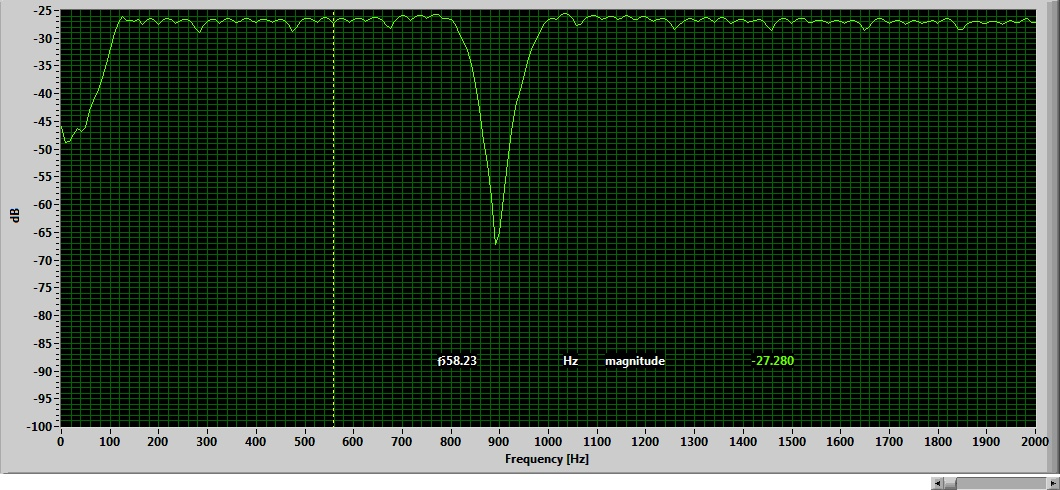
\includegraphics[width=0.80\textwidth]{IIRrealisatie}\par\vspace{1cm}
    Wanneer er een probleem zou zijn met een IIR filter is dat meteen zichtbaar omdat het filter zich dan totaal niet gedraagd zoals gewenst is, maar in dit geval ziet u duidelijk dat hij overheen komt met de voorspelling van Matlab.
    
\clearpage

	\section{Optimalisatie}
	De enige optimalisaties is uitgevoerd heeft niets te maken met de prestaties tijdens het uitvoeren op de EzDSP. Alleen is de leesbaarheid van de code verbeterd doordat de staat van de filters in een struct wordt bijgehouden. Er zijn functies beschreven die iets in de buffer op kunnen slaan of een output sample kunnen berekenen. Hierdoor is de code ook beter herbruikbaar. 
	
 
	\section{Conclusie en aanbevelingen}
	Tijdens TDS word er aardig wat wiskunde gebruikt. Dit moet ook worden gebruikt tijdens het progammeren. Dit kwam in het begin vrij intimiderend over. De eerste vier opgaven waren bij lange na niet zo moeilijk als 5 en 6. 
	Het ontwikkelen van een FIR filter viel achteraf nog erg mee vergeleken met het ontwikkelen van het IIR filter, dit kwam vooral omdat fouten niet meteen duidelijk waren bij een FIR filter. Kleine foutjes hadden namelijk een kleine invoud op de uitvoer. 
	Bij IIR zorgte ieder kleine foutje ervoor dat het filter niet werkte. Dit komt omdat de uitvoer tijdens het ene output sample weer werd meegenomen in de berekening van het volgende output sample.

	De laatste week dat we de tijd hadden om de opgaven 6a en 6b af te laten tekenen is het realiseren van een single section IIR filter gelukt. Hierna was geen tijd meer om een filter met meerdere secties te realiseren.
	Het filter dat gerealiseerd hoordde te worden was vrij complex en niet goed realiseerdbaar met een single section filter. Met de docent is daarom besproken om de eisen van ons filter iets te verlagen, ten kosten van het eindcijfer. Met meer tijd had het wel gelukt om dit filter volledig te realiseren. 
	\bibliographystyle{plain}
	\bibliography{bibligraphy}
		
	\begin{thebibliography}{9}

	\bibitem{analog}
  		
  		\textit{A Beginner's Guide to Digital Signal Processing (DSP)},
  		Analog Devices,
  		URL: http://www.analog.com/en/design-center/landing-pages/001/beginners-guide-to-dsp.html 
  		
	\bibitem{DSPguide}
  		
  		\textit{Scientist and Engineer's Guide to Digital Signal Processing},
  		Steven W. Smith, Ph.D., 
  		Bertrams,
  		Hoofdstuk 14,
  		1998.  		
		
	\end{thebibliography}

\end{document}